\documentclass{article}
\usepackage[utf8]{inputenc}
\usepackage[export]{adjustbox}
\usepackage{subfigure}
\usepackage{url}
\usepackage{graphicx}
\graphicspath {
	{images/}
}

\begin{document}

\title{Prototyping}
\author{Cardspark - Group 26}
\date{\today}
\maketitle

Before we started the implementation of our app, we created a digital prototype that allowed us and the users to navigate through it as if it were an actual mobile application.  We did this using FluidUI and we passed this link to many potential users of the app and in turn they gave us feedback and areas of improvement.

\begin{figure}[ht]
	\centering
	\begin{subfigure}{}
	  \centering
			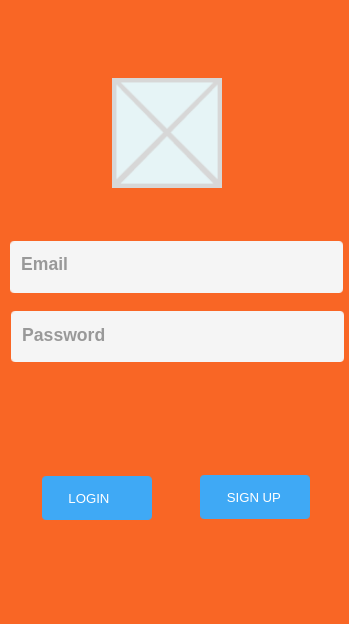
\includegraphics[scale=0.25]{fluidlogin.png}
	\end{subfigure}%
	\begin{subfigure}{}
	  \centering
			
\includegraphics[scale=0.25]{fluidcard.png}
	\end{subfigure}
\end{figure}

Here's how the prototype views were put together in storyboard.
\begin{center}
	\vspace{1mm}
	
\includegraphics[scale=0.2]{placeholder.png}
	\vspace{1mm}
\end{center}

\newpage

During the technical implementation of our application, we made use of iOS phones to demo our app and allow ourselves and other users to test the app and therefore look for improvements.  As you can see below, our storyboard at this stage has become a lot more complex, with additions and changes due to to user feedback as well as new ideas being implemented.

Changes such as changing the layout of the login screen that now conforms with the typical iOS layout that users are used to.  Our friends mentioned that the previous prototype was very strict in that the image must go in one place and that one big section of text should go here.

\begin{center}
	\vspace{1mm}
	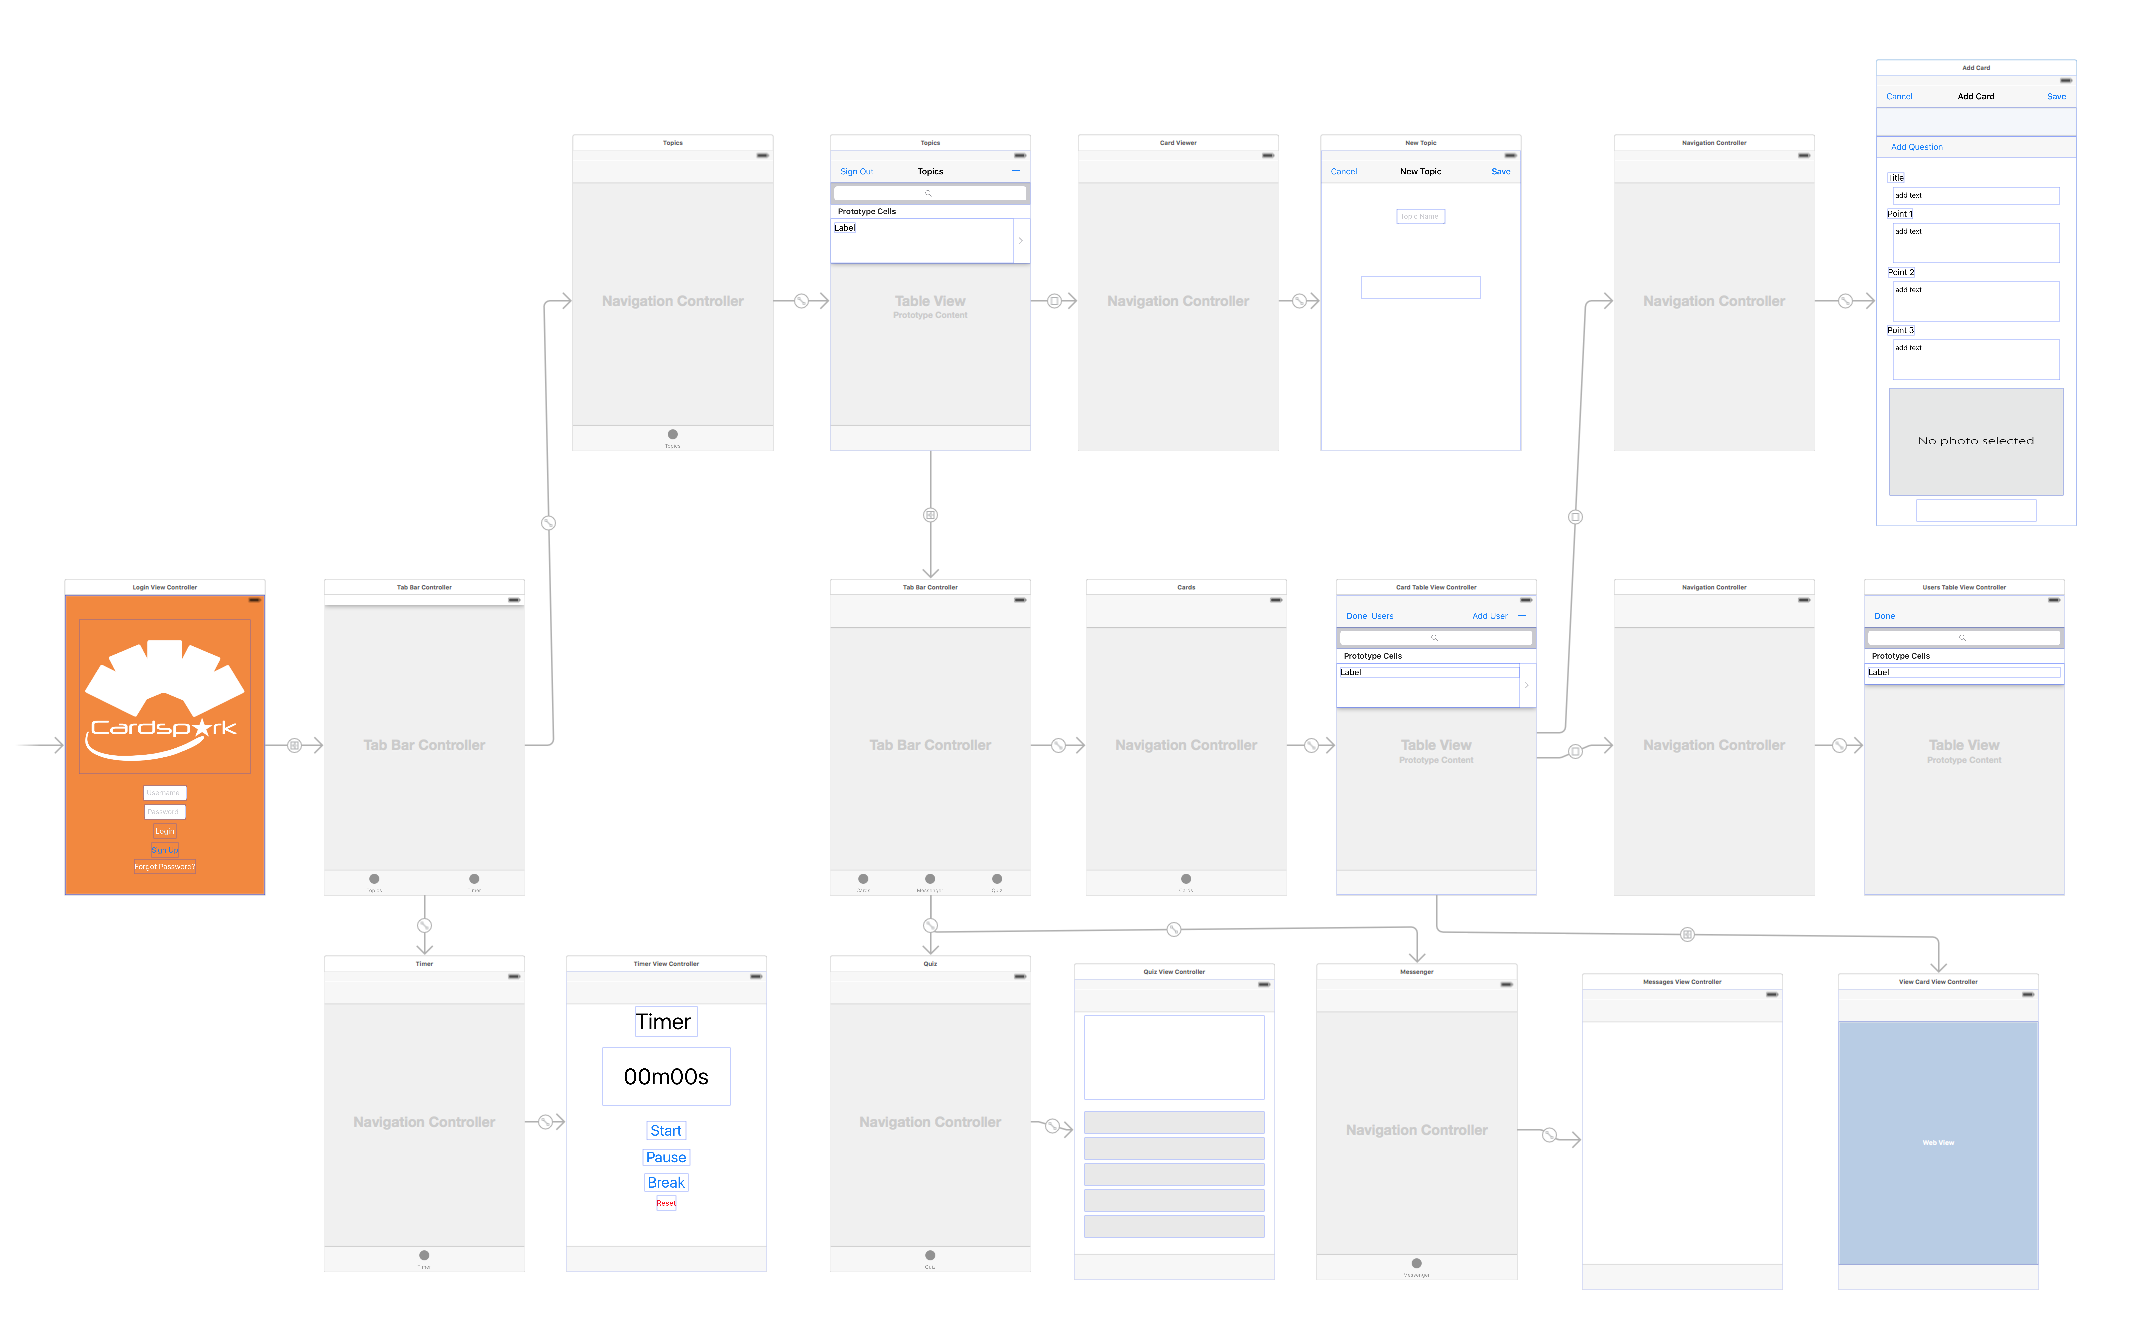
\includegraphics[scale=0.3]{storyboard.png}
	\vspace{1mm}
\end{center}

Here is a user using a prototype that we have placed on an iOS phone.	

\begin{figure}[ht]
	\centering
	\begin{subfigure}{}
	  \centering
			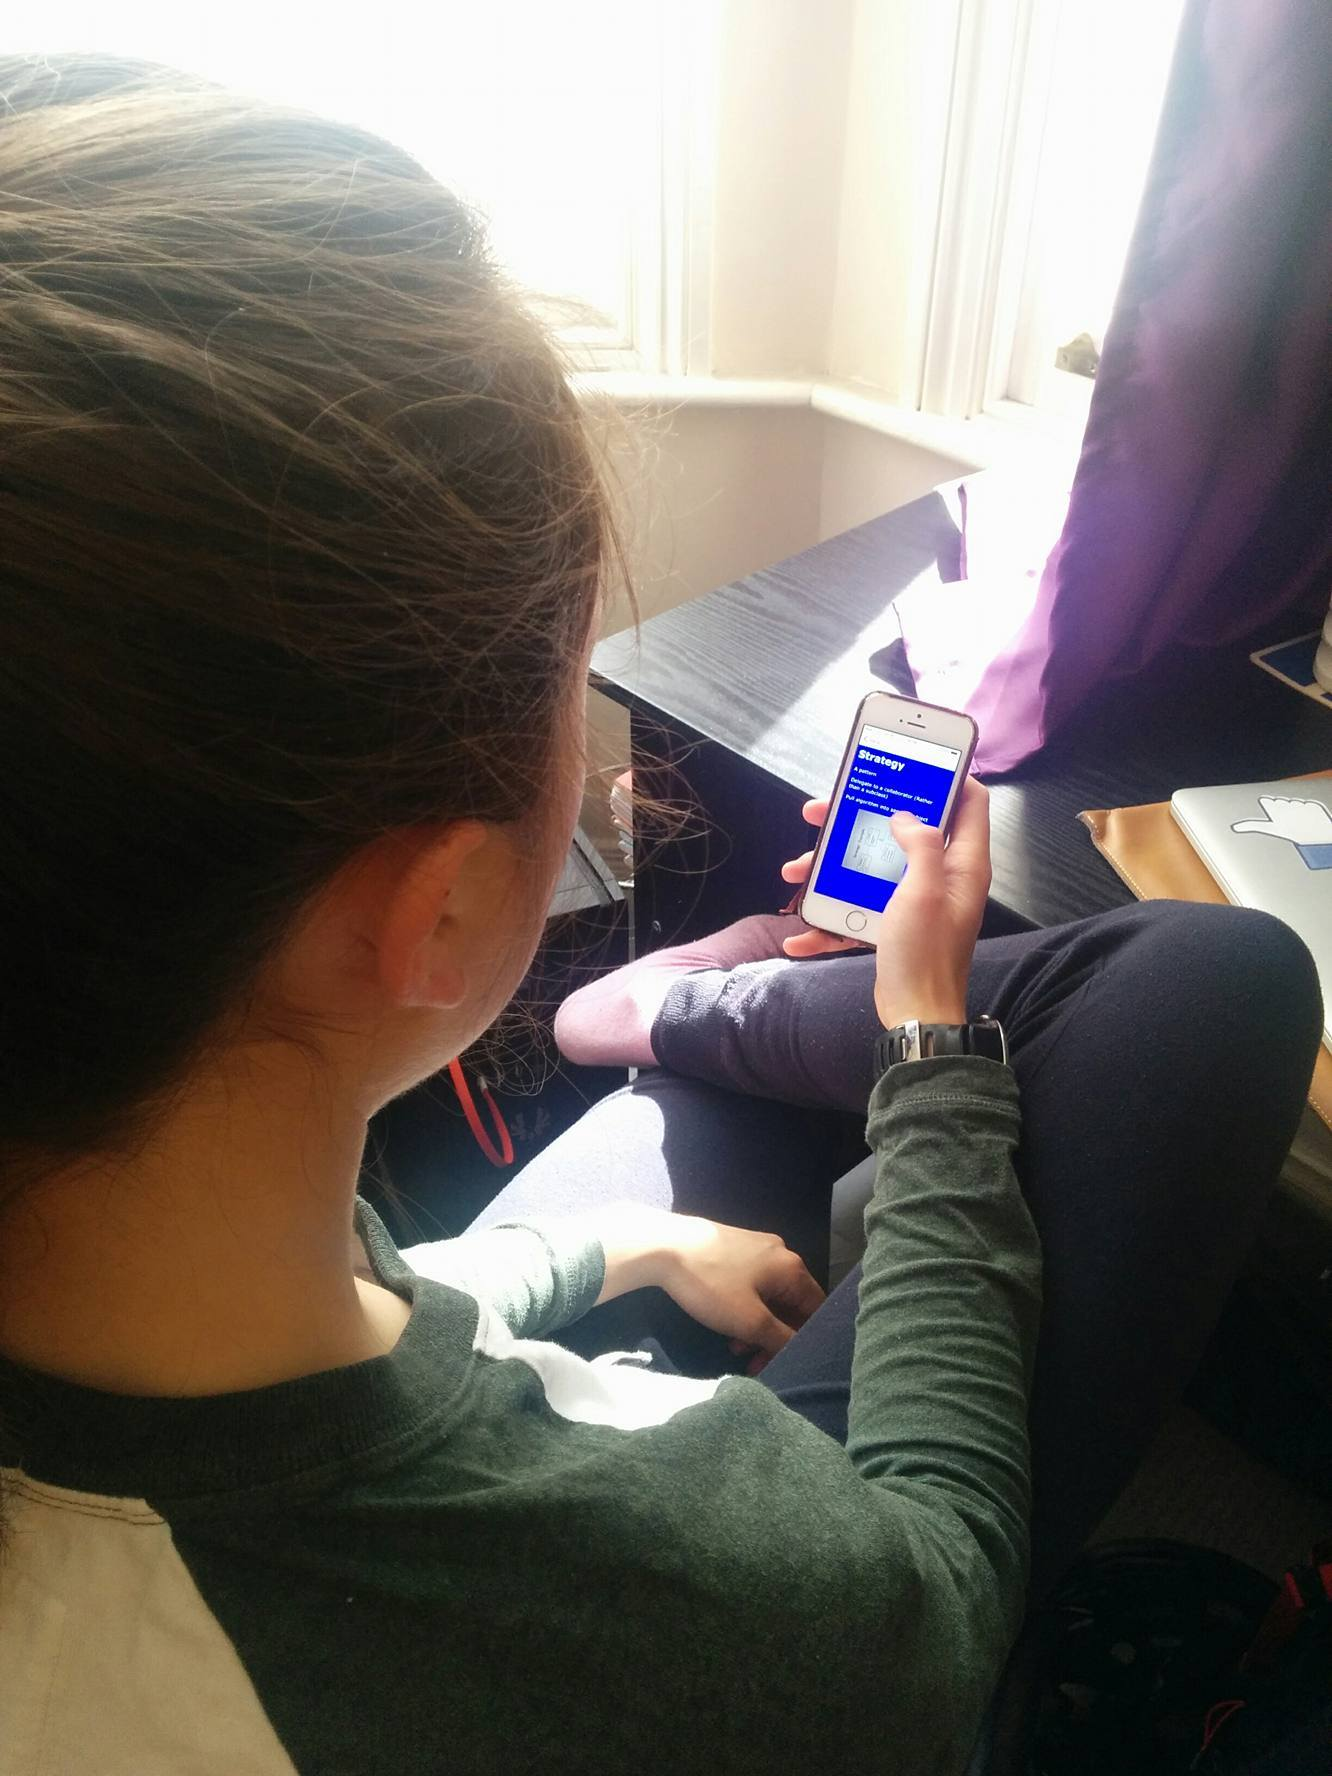
\includegraphics[scale=0.1]{prototype_use.jpg}
	\end{subfigure}%
	\begin{subfigure}{}
	  \centering
			
\includegraphics[scale=0.1]{prototype_swipe.jpg}
	\end{subfigure}
\end{figure}



\end{document}
